In this section, we show empirical results of our algorithm for different transferring situations on two image benchmark datasets: Office and Caltech.
\subsection{Dataset \& Baseline methods}
Office contains 31 classes from 3 subsets (Amazon,Dslr and Webcam) and Caltech contains 256 classes. We select 13 shared classes from two datasets\footnote{13 classes include: backpack, bike, helmet, bottle, calculator, headphone, keyboard, laptop, monitor, mouse, mug, phone and projector}. The input features of all examples are extracted using AlextNet\cite{krizhevsky2012imagenet}.
Because the two subsets Dslr and Webcam are relatively small and don't have data for testing, we don't use them as our target domain.

We compare our algorithm SMTLe with two kinds of baselines. The first one is the methods without leveraging any prior knowledge (no transfer baselines). \textbf{No transfer:} SVMs trained only on target data. Any transfer algorithm that performs worse than it suffers from negative transfer. \textbf{Batch:} We combined the source and target data, assuming that we have full access to all data, to train the SVMs. The result of the Batch method might be considered as the best performance achieved during the transfer learning. The second kind of baseline consists of two previous transfer methods in HTL, \textbf{MKTL\cite{jie2011multiclass}} and \textbf{Multi-KT\cite{tommasi2014learning}}. Similar to SMTLe, both of them use the LOOCV method to estimate the relatedness of the source model and target domain, but they use their own convex objective function without the $\ell_2$ penalty terms. 
\subsection{Extensive experiments on benchmarks}
In this subsection, we perform 6 groups of experiments under the setting of HTL. In each group of experiment, the source model is trained using linear SVMs on the whole source data. We use 5 different sizes of training data for each class in the target domain. Experiment results are reported by averaging over 10 rounds and shown in Figure \ref{fig:exp}. 

\textbf{Observation \& discussion:} SMTLe can significantly outperform other baselines especially when the training size is small. Moreover, in some groups of experiments, they even suffer from negative transfer on the small training set. As we discussed above, without the $\ell_2$ penalty in the objective functions when the training set is small, these two HTL baselines are not able to estimate the relatedness between the source model and target domain well. However, as the training size increases, the variance of the estimation of LOOCV decreases. The affect of the $\ell_2$ penalty term become less significant. Meanwhile, the target data contains more useful information to learn a better target model. Therefore, SMTLe and the other two HTL baselines show similar performance. In some experiments, it is interesting to see that SMTLe can even outperform the Batch method which might be considered as the the best performance under the setting of HTL.
\begin{figure}[th]
\centering
\subfigure[C$\rightarrow$A]{
    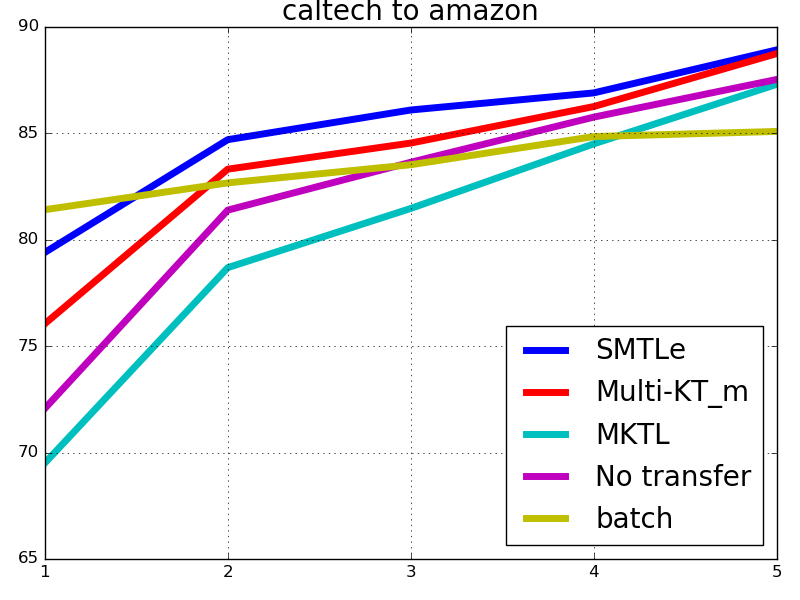
\includegraphics[width=0.22\textwidth]{fig/caltechtoamazon.png}\label{a}
}
\subfigure[D$\rightarrow$A]{
    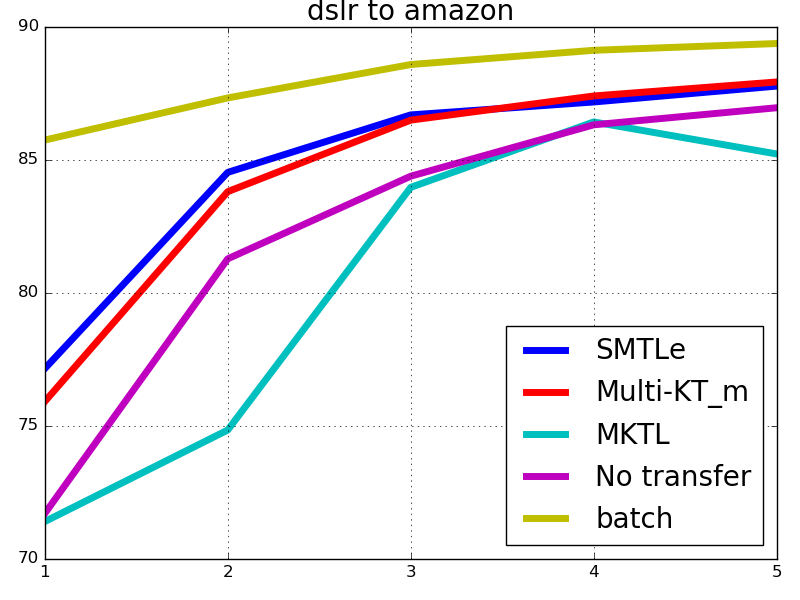
\includegraphics[width=0.22\textwidth]{fig/dslrtoamazon.png}\label{b}
}
\subfigure[W$\rightarrow$A]{
	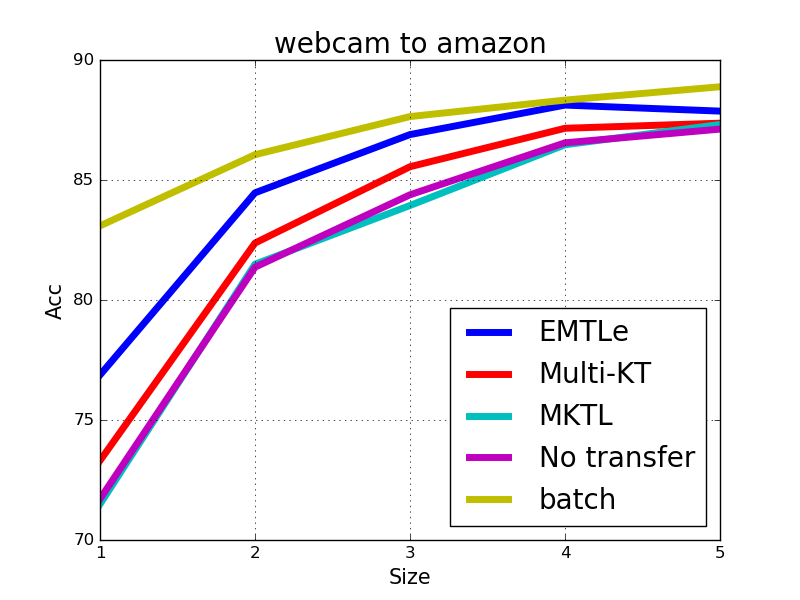
\includegraphics[width=0.22\textwidth]{fig/webcamtoamazon.png}\label{c}
}
\subfigure[A$\rightarrow$C]{
	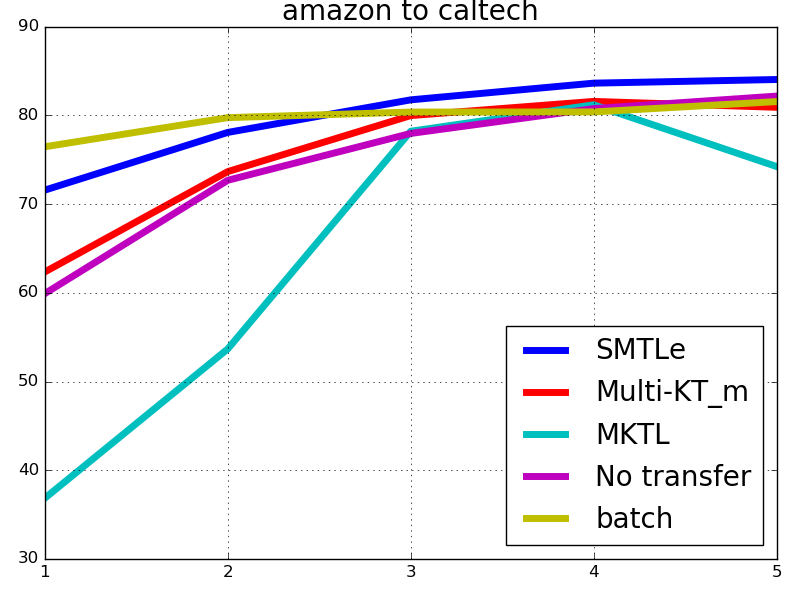
\includegraphics[width=0.22\textwidth]{fig/amazontocaltech.png}\label{d}
}\\
\subfigure[D$\rightarrow$C]{
	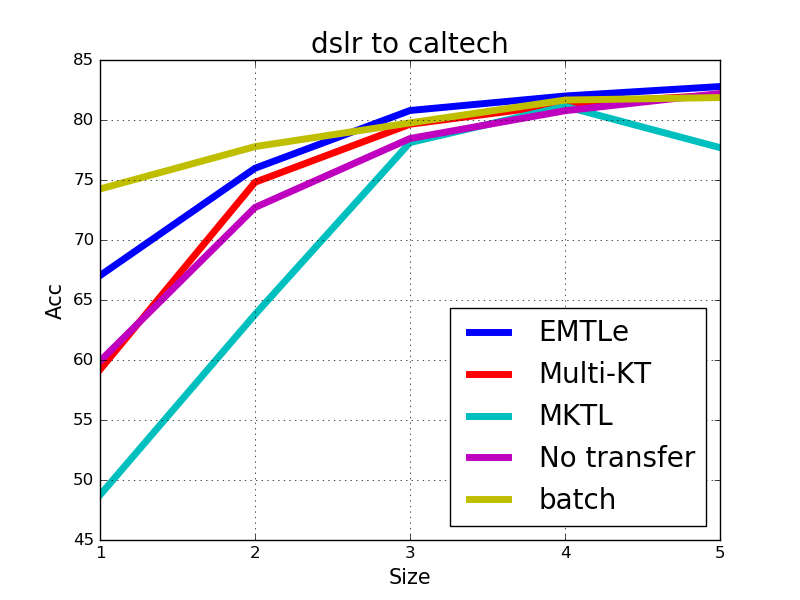
\includegraphics[width=0.22\textwidth]{fig/dslrtocaltech.png}\label{e}
}
\subfigure[W$\rightarrow$C]{
	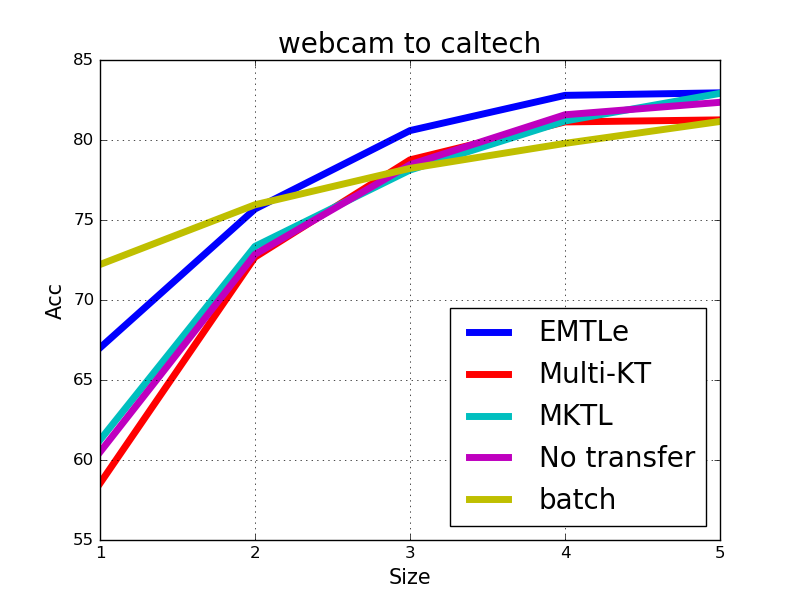
\includegraphics[width=0.22\textwidth]{fig/webcamtocaltech.png}\label{f}
}
\subfigure[A$\rightarrow$D]{
	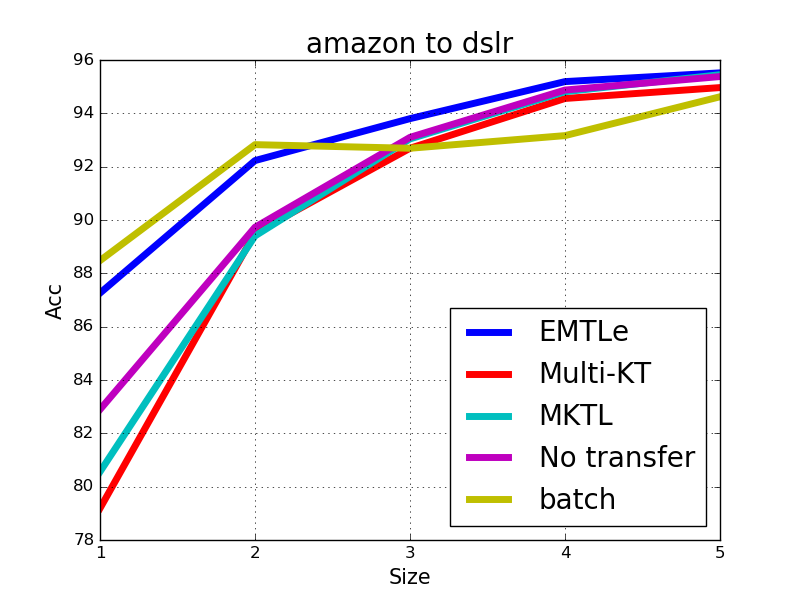
\includegraphics[width=0.22\textwidth]{fig/amazontodslr.png}\label{g}
}
\subfigure[C$\rightarrow$D]{
	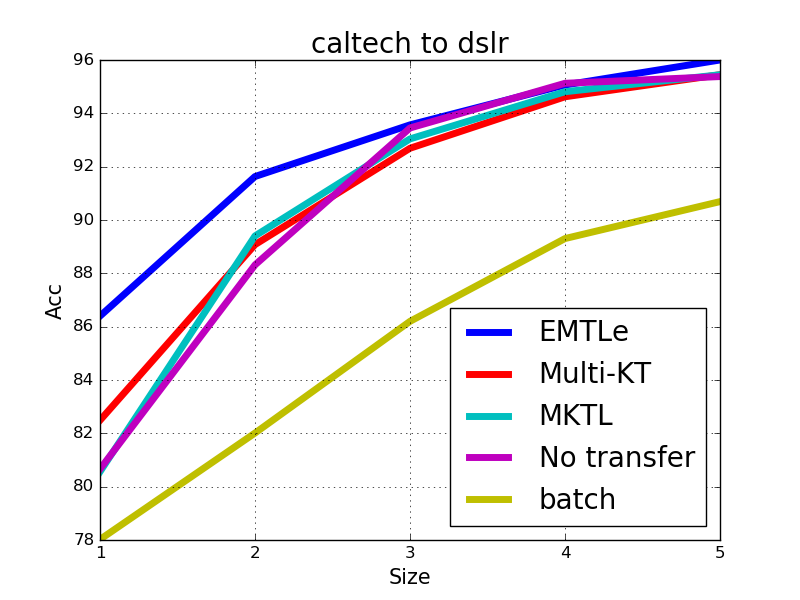
\includegraphics[width=0.22\textwidth]{fig/caltechtodslr.png}\label{h}
}\\
\subfigure[W$\rightarrow$D]{
	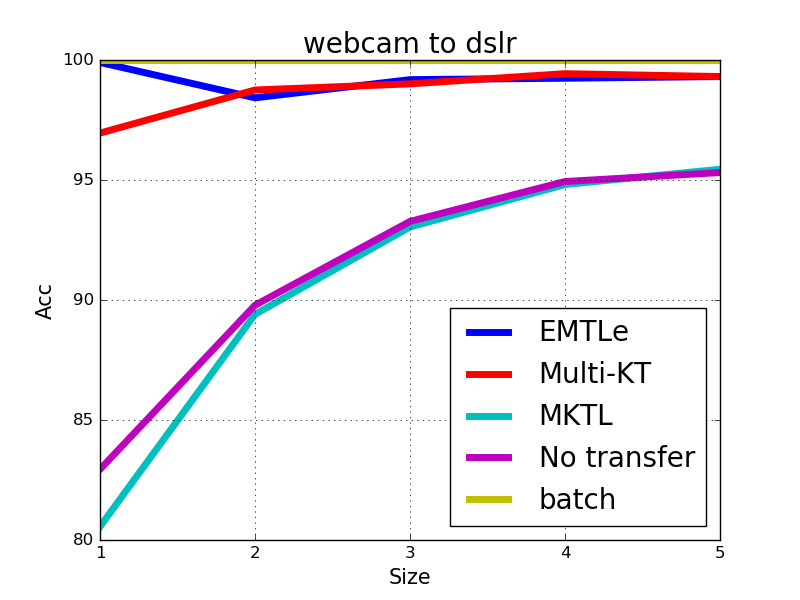
\includegraphics[width=0.22\textwidth]{fig/webcamtodslr.png}\label{i}
}
\subfigure[A$\rightarrow$W]{
	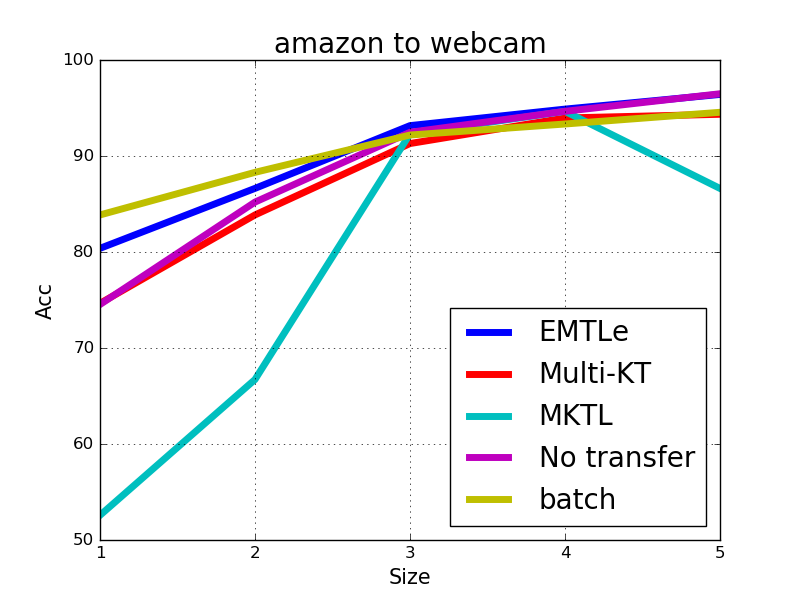
\includegraphics[width=0.22\textwidth]{fig/amazontowebcam.png}\label{j}
}
\subfigure[C$\rightarrow$W]{
	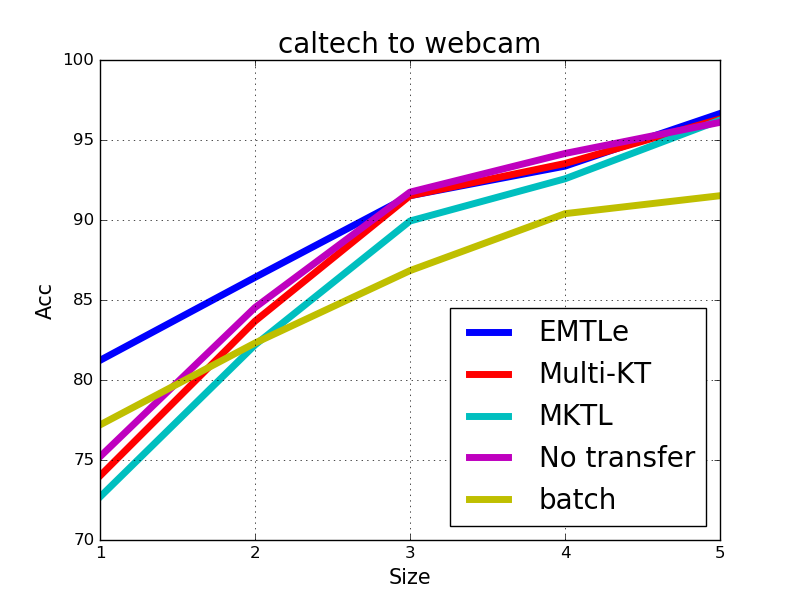
\includegraphics[width=0.22\textwidth]{fig/caltechtowebcam.png}\label{k}
}
\subfigure[D$\rightarrow$W]{
	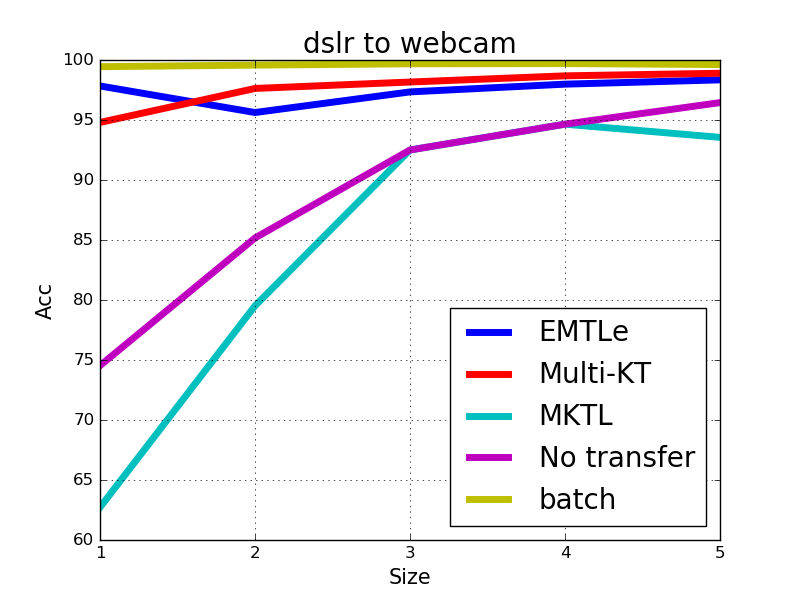
\includegraphics[width=0.22\textwidth]{fig/dslrtowebcam.png}\label{l}
}
\caption{Recognition accuracy for HTL domain adaptation from a single source. 5 different sizes of target training sets are used in each group of experiments.}
\label{fig:exp}
\end{figure}

\textbf{Observation \& discussion:} EMTLe can significantly outperform other baselines especially with a small training set. %Moreover, in some groups of experiments, they even suffer from negative transfer on the small training set. 
As we have discussed above, when the training set is small, with the transfer parameter estimated by our $\ell_2$ penalty in our high-level objective functions, EMTLe has a strong generalization ability and performs better on the test data. As the training size increases, the variance of training data decreases and the affect of the $\ell_2$ penalty term become less significant. Therefore, EMTLe and the other two HTL baselines show similar performance. 
It is interesting to see that MKTL even falls into negative transfer even with 5 training examples per class in some experiments. We found that, MKTL is more sensitive to the variance of the training data. Its performance is not as stable as Multi-KT and EMTLe over the 10 experiments. Because MKTL needs to learn more hyperparameters than Multi-KT and EMTLe, even though the training size increases, it may not be able to obtain a good model. 
In some experiments, we can see that EMTLe can even outperform the Batch method which can access more information and is expected to outperform the other methods under the setting of HTL.


